\documentclass[xcolor=dvipsnames]{beamer} 
\usepackage{booktabs}
\usepackage{bm}
\usepackage{multicol}
\usepackage{amssymb}

\newcommand{\beqa}{\begin{eqnarray*}}
\newcommand{\eeqa}{\end{eqnarray*}}

\usepackage{setspace}
\usepackage{longtable}
\usepackage{xcolor}
\usepackage{lscape}
\usepackage{dcolumn}
\usepackage{booktabs}

\newcommand{\mbfy}{{\mathbf y}}
\newcommand{\mbfx}{{\mathbf x}}
\newcommand{\mbfX}{{\mathbf X}}

\usepackage{colortbl}
 \setbeamercolor{title}{fg=WUSTLgreen, bg=WUSTLtan}
\newcommand{\gray}[1]{\color{gray}{#1}}
\newcommand{\grayTwo}[1]{\color{grayTwo}{#1}}


\usepackage{tikz}


\usetikzlibrary{shapes.geometric, arrows,fit,positioning}
\tikzstyle{user} = [rectangle, minimum width=1cm, minimum height=2cm,text centered, draw=black, fill=red!30]
\tikzstyle{turker} = [rectangle, minimum width=1cm, minimum height=2cm,text centered, draw=black, fill=green!30]
\tikzstyle{comp} = [rectangle, minimum width=1cm, minimum height=2cm,text centered, draw=black, fill=blue!30]

\tikzstyle{arrow} = [thick,->,>=stealth]
\tikzstyle{arrow2} = [thick,->,>=stealth]


\usetheme[]{Boadilla} 

\definecolor{WUSTLgreen} {RGB} {44, 80, 54}
\definecolor{WUSTLred} {RGB} {149, 1, 1}
\definecolor{WUSTLtan} {RGB} {229, 210, 184}
\setbeamercolor{structure}{fg=WUSTLred, bg=WUSTLgreen}
\setbeamercolor{normaltext}{bg=black, fg=WUSTLtan}
\setbeamercolor{block title}{fg=WUSTLred}
\setbeamercolor{block title example}{fg=WUSTLgreen}
\setbeamercolor{frametitle}{fg=WUSTLgreen}
\setbeamercolor{title}{fg=WUSTLgreen}



\setbeamertemplate{blocks}[rounded]

\usepackage{graphicx}
\usepackage{amsmath}
\usepackage{multirow, multicol}
\usepackage{mathpazo}
\usepackage{amsthm}
\usepackage{amssymb}
\usepackage{setspace}
\usepackage{hyperref}
\usepackage{array,colortbl,booktabs}
\usepackage{soul}

\newtheorem{blank}{}
\newtheoremstyle{mystyle}% name of the style to be used
 {}% measure of space to leave above the theorem. E.g.: 3pt
  {}% measure of space to leave below the theorem. E.g.: 3pt
  {}% name of font to use in the body of the theorem
  {20pt}% measure of space to indent
  {}% name of head font
  {}% punctuation between head and body
  {}% space after theorem head; " " = normal interword space
  {}% Manually specify head

\newcommand{\bframe}{\begin{frame}}
\newcommand{\jacob}{\end{frame}}
\newcommand{\bi}{\begin{itemize}}
\newcommand{\ei}{\end{itemize}}
\newcommand{\be}{\begin{enumerate}}
\newcommand{\ee}{\end{enumerate}}
\newcommand{\vp}{\vspace{.5cm}}
\newcommand{\bis}{\begin{itemize}[<+->]}
\newcommand{\bes}{\begin{enumerate}[<+->]}
\newcommand{\red}[1]{\color{WUSTLred}{#1}}
\newcommand{\bc}{\begin{center}}
\newcommand{\ec}{\end{center}}
\newcommand{\eb}{\end{block}}









\graphicspath{{../LectureGraphics/}}
\DeclareGraphicsExtensions{.pdf,.png,.jpg,.jpeg,.mps}






% \newcommand{\bis}{\begin{itemize}[<+->]}
% \newcommand{\bi}{\begin{itemize}}
% \newcommand{\ei}{\end{itemize}}


\newcommand{\skipslide}{\addtocounter{framenumber}{-1}}

\title[EBMA]{Bayesian Model Averaging}
\author[Montgomery ]{Jacob M. Montgomery \vspace{-.4cm}}
\institute[Wash U.]{\gray Department of Political Science, Washington University in St. Louis}
\date[November 11, 2016]{}


\setbeamertemplate{navigation symbols}{}
\begin{document}


%\subsection{ }
\frame{\titlepage}


\begin{frame}
\frametitle{Too many variables, not enough theory}

Fearon and Laitin (2003) wish to model civil conflict
\begin{center}
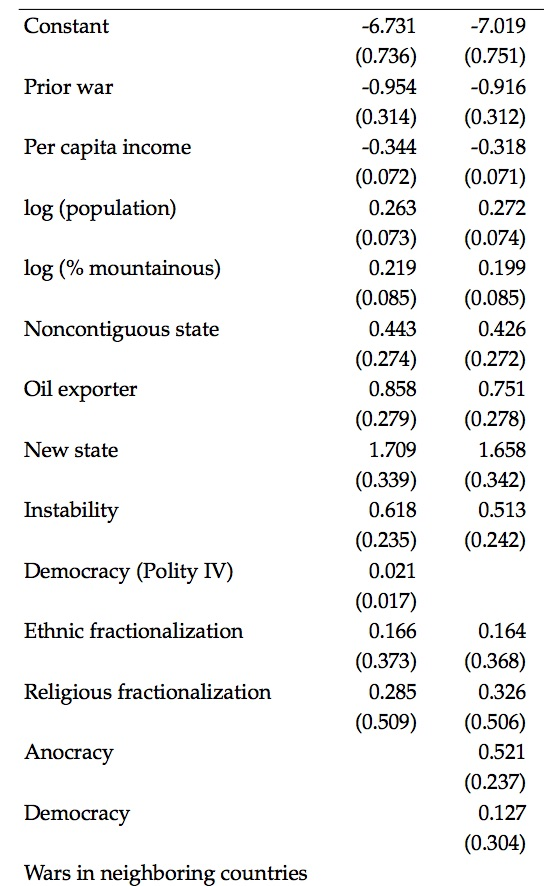
\includegraphics[scale=.18]{model}
\end{center}

\end{frame}


\begin{frame}
\frametitle{Too many variables, not enough theory}

\begin{quote}
``When we add dummy variables for countries that have
an ethnic or religious majority and a minority of at least
8\% of the country’s poulation, both are incorrectly signed
and neither comes close to statistical significance. \textit{This
finding does not depend on which other variables are included
in the model}.''
\end{quote}

\vp
We often want to show that our results are ``robust'' to modeling
choices:
\pause
\bis
\item Online appendix includes 18 additional tables
\item At least 74 possible explnatory variables discussed
\item $2^{74}=2\times10^{22}=20 sextillion$
\item Our actual uncertainty vastly understated
\ei

\end{frame}


\begin{frame}
\frametitle{Bayesian model averaging}

The setup:
\bi
\item $Y$ is a $n \times 1$ vector of outcomes
\item $X$ is an $n \times p$ matrix
\item $Y = X\beta + \epsilon$
\item $\epsilon \sim N(0, \sigma^2 I)$
\item $q=2^p$
\item $\mathcal{M}=[\mathcal{M}_1, \mathcal{M}_2,\ldots,\mathcal{M}_q ]$
\ei


\end{frame}


\begin{frame}
\frametitle{Bayesian model averaging}

Priors and likelihood:
\bi
\item $\mathcal{M}_k \sim \pi(\mathcal{M}_k)$
\item $\sigma^2|\mathcal{M}_k \sim \pi(\sigma^2|\mathcal{M}_k)$
\item $\beta_\omega|\sigma^2, \mathcal{M}_k \sim
  \pi(\beta_\omega|\sigma^2, \mathcal{M}_k)$
\item $\Omega=[\omega_1, \ldots, \omega_p]$ is a binary vector
  indicating inclusion.
\ei

\vp \pause
$$p(Y|\beta_\omega, \sigma^2, \mathcal{M}_k) \sim
N(X_\omega\beta_\omega, \sigma^2I) $$

\vp \pause
$$p(Y| \mathcal{M}_k) \sim \int \int  p(Y|\beta_\omega, \sigma^2,
\mathcal{M}_k) \pi(\beta_\omega|\sigma^2, \mathcal{M}_k)
\pi(\sigma^2|\mathcal{M}_k) d\beta_\omega d\sigma^2$$



\end{frame}




\begin{frame}
\frametitle{Bayesian model averaging}

$$P(\mathcal{M}_k|Y) = \frac{p(Y| \mathcal{M}_k) \pi(\mathcal{M}_k)}{\sum_kp(Y| \mathcal{M}_k) \pi(\mathcal{M}_k)} $$

\vp \pause
With this, we can easily create other quantities of interest as
weighted sums. For example,  
$$E(\beta_k |Y) = \sum_{k=0}^q P(\mathcal{M}_k|Y) E(\beta|M_k,Y) $$

\end{frame}


\begin{frame}
\frametitle{Bayesian model averaging}

$$P(\mathcal{M}_k|Y) = \frac{p(Y| \mathcal{M}_k) \pi(\mathcal{M}_k)}{\sum_kp(Y| \mathcal{M}_k) \pi(\mathcal{M}_k)} $$

\vp \pause
With this, we can easily create other quantities of interest as
weighted sums. For example,  
$$E(\beta_k |Y) = \sum_{k=0}^q P(\mathcal{M}_k|Y) E(\beta|M_k,Y) $$

\end{frame}

\begin{frame}
\frametitle{What do we get?}

\begin{center}
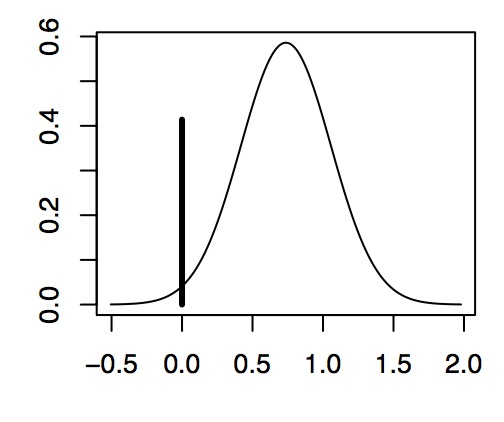
\includegraphics[scale=.3]{Figure}
\end{center}

\begin{enumerate}
\item Does the variable contribute to the model’s explanatory power?
(i.e. what is the posterior probability of all models that include
this variable?)
\item  Is it correlated with unexplained variance when it is included?
(i.e. what is the conditional posterior distribution assuming
that the variable is included?)
\end{enumerate}


\end{frame}

\begin{frame}
\frametitle{Practical and technical notes}

\bis
\item Can constrain model space in motivated ways
\item Can reformulate the posterior for each model probability as:
$$P(\mathcal{M}_k|Y) = \frac{p(Y| \mathcal{M}_k) \pi(\mathcal{M}_k)/p(\mathcal{M}_0|Y)\pi(\mathcal{M}_0)}{\sum_kp(Y| \mathcal{M}_k) \pi(\mathcal{M}_k) \pi(\mathcal{M}_k)/p(\mathcal{M}_0|Y)\pi(\mathcal{M}_0)} $$ 
\item Also need a prior on the model space:
$\pi(\mathcal{M}_k) = \gamma^{p_\omega}(1-\gamma)^{p-p_\omega}$
\item Can even put a hyperprior on $\gamma$
\ei

\end{frame}

\frame { \frametitle{Prior Selection}

The limiting factor in BMA approaches has always been a combination
of:
\begin{itemize}
\item an \emph{extremely} high dimensional space
\item intractable integrals.
\end{itemize}

Early work used ``approximations'' of the Bayes factors as a
solution:
\begin{itemize}
\item $BIC_k = -2\mbox{log}(L_k-L_0)+p_k\mbox{log}n$
\item $AIC_k = -2\mbox{log}(L_k-L_0)+2p$
\end{itemize}

}

\frame { \frametitle{Newer alternatives}

Clyde (2003) and Clyde and George(2004) summarize a more
comprehensive approach.
\begin{equation}\label{int}
\pi(\mathcal{M}_k)=\gamma^{p_\omega}(1-\gamma)^{p-p_\omega}
\end{equation}

\begin{flushleft}
\begin{tabular}{lll}
\multicolumn{3}{l}{\textbf{Priors for posterior calculations}}\\
\emph{Prior} & \emph{Formulation} &  \\
\hline { $g$-prior} & $\pi(\beta_\omega|\mathcal{M}_k,\sigma^2) \sim
N_{p_\omega}(0,g \sigma^2(X_\omega'X_\omega)^{-1})$ & \\
& $\pi(\beta_0, \sigma^2 | \mathcal{M}_k) \propto 1/\sigma^2$ & \\

\hline
\\
\multicolumn{3}{l}{\textbf{Hyper-priors for $g$}}\\
\emph{Prior} & \emph{Formulation} &  \\
\hline {\footnotesize Hyper-$g$}&  $\pi (g) = \frac{a-2}{2}
(1+g)^{\frac{a}{2}} \, \mathrm{if} g > 0$
&\\
{\footnotesize ZS} & $\pi(g)=\frac{(n/2)^{1/2}}{\Gamma(1/2)}
g^{-3/2}e^{-\frac{n}{2g}}$ & \\
\hline
\end{tabular}
\end{flushleft}

\normalsize
 }



\begin{frame}

\centering
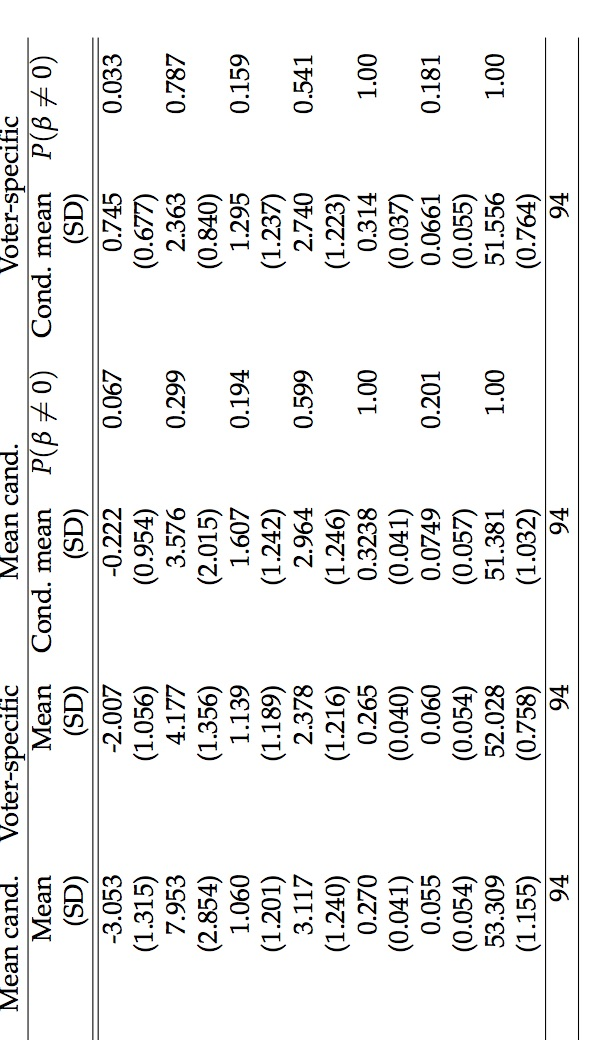
\includegraphics[angle=270, scale=.3]{Table}

\end{frame}

\begin{frame}
\frametitle{Improving forecasting with BMA}

\bi
\item We often have many forecasting models for specific outcomes
\item Not all of them are equally valuable, and not all provide unique
  insight
\item Can we combine forecasts to reduce model dependency and improve
  our out-of-sample performance?
\ei

\end{frame}


\begin{frame}
\frametitle{Improving forecasting with BMA}

The setup:
\bis
\item $\mathbf{y}^{t\ast}$ are outcomes in the future we want to
  predict.
\item $\mathbf{y}^{t}$ are outcomes in the past that we previously
  tried to predict (out of sample)
\item We have $K$ forecasting models or teams, $M_1, M_2, \ldots, M_K$.
\ei

\end{frame}


\begin{frame}
\frametitle{Improving forecasting with BMA}

The punchline
\bis
\item $M_k \sim \pi(M_k)$
\item Pdf for the forecast is $p(\mathbf{y}^t |M_k)$
\item $$p(M_k | \mathbf{y}^t)  =
  \frac{p(\mathbf{y}^t|M_k)\pi(M_k)}{\sum_k
    p(\mathbf{y}^t|M_k)\pi(M_k)}$$
\item $$p(\mathbf{y}^{t\ast}) = \sum
  p(\mathbf{y}^{t\ast}|M_k)p(M_k|\mathbf{y}^t)$$
\item $$E(\mathbf{y}^{t\ast}) = \sum E(\mathbf{y}^{t\ast}|M_k)p(M_k|\mathbf{y}^t)$$

\ei

\end{frame}





\frame{
\frametitle{EBMA as a finite mixture model}

\bi
\item Denote $w_k=p(M_k|\mathbf{y}^t)$
\item Let $p(\mathbf{y}^{t^*}|M_k)=N(f_k^{t^\ast}, \sigma^2)$
\ei


\begin{equation}
\label{pdf}p(y|f_1^{s|t^\ast},
\ldots, f_K^{s|t^\ast}) = \overset{K}{\underset{k=1}{\sum}} w_k
N(f_k^{t^\ast}, \sigma^2).
\end{equation}

\begin{equation}
\mathcal{L}(\mathbf{w}, \sigma^2)=\sum_t\log\left(\sum_{k=1}^Kw_kN(f^t_k, \sigma^2) \right),
\end{equation}



}

\begin{frame}
\frametitle{E-M Algorithm}

\begin{equation}
\label{E-step}
\hat{z}^{(j+1)t}_{k} = \frac{\hat{w}^{(j)}_k
p^{(j)}(y|f_{k}^{t})}{\overset{K}{\underset{k=1}{\sum}}\hat{w}^{(j)}_kp^{(j)}(y|f_{k}^{t})},
\end{equation}


\begin{equation}
\label{M-step}
\hat{w}^{(j+1)}_k=\frac{1}{n}\underset{t}{\sum}\hat{z}^{(j+1)t}_{k},
\end{equation}


\end{frame}

\begin{frame}
\frametitle{Example: Predicting presidential elections}

\bi
\item \textbf{Campbell}: Campbell’s “Trial-Heat and Economy Model” 
\item \textbf{Abramowitz}: The “Time-for-Change Model” created by ?
\item \textbf{Fair}: Fair’s presidential vote-share model16
\item \textbf{Lewis-Beck/Tien}: Lewis-Beck and Tien’s “Jobs Model Forecast” 
\item \textbf{EW}: Erikson \& Wlezien,
\ei
\end{frame}



\begin{frame}
\frametitle{Previous performance}

\centering
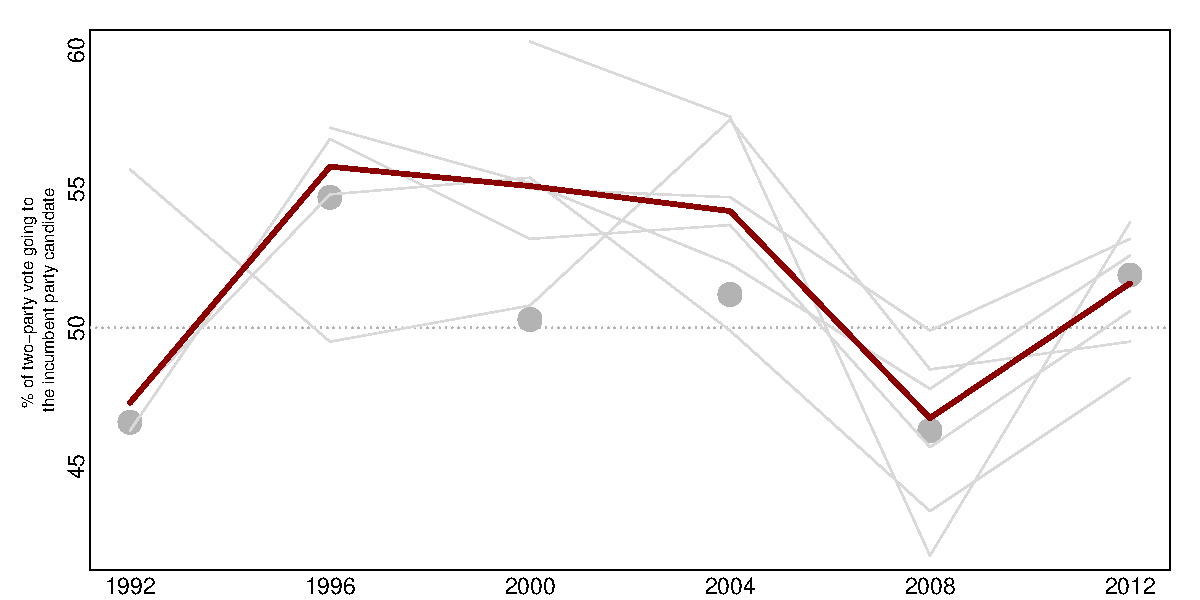
\includegraphics[scale=.6]{PotentialGraph}

\end{frame}

\begin{frame}
\scriptsize
\begin{center}
\begin{tabular}{l rrrrrrrr}	
  \toprule
   &\multicolumn{4}{c}{\textit{2004 Election}} &\multicolumn{4}{c}{\textit{2008 Election}} \\ 
 &	Weights&	RMSE &MAE &\shortstack{Pred. \\ Error}
 &Weights&	RMSE&	MAE &  \shortstack{Pred.\\  Error}\\
\midrule
 Campbell               &0.40&1.71&1.33 &0.53&0.36&1.65&1.28&6.33\\
  Abramowitz        	&0.00&1.50&1.18&2.20&0.06&1.53&1.26&$-$2.37\\
  Hibbs                   	&0.12&1.95&1.38&1.54&0.25&1.92&1.38&$-$1.39\\
  Fair                      	&0.48&2.07&1.47&4.82&0.00&2.22&1.80&$-$2.02 \\
  Lewis-Beck/Tien 	&0.00&1.67&1.42&$-$0.41&	0.17&1.61&1.33&$-$2.65\\
  Erikson/Wlezien 	&0.00&2.67&2.06&4.76&0.17&2.81&2.18&$-$0.14\\
   EBMA                    	&	       	&1.29&1.01&2.08&
  &1.30&1.01&$-$0.53\\
\bottomrule
\end{tabular}
 \end{center}
\end{frame}



\begin{frame}

\begin{center}
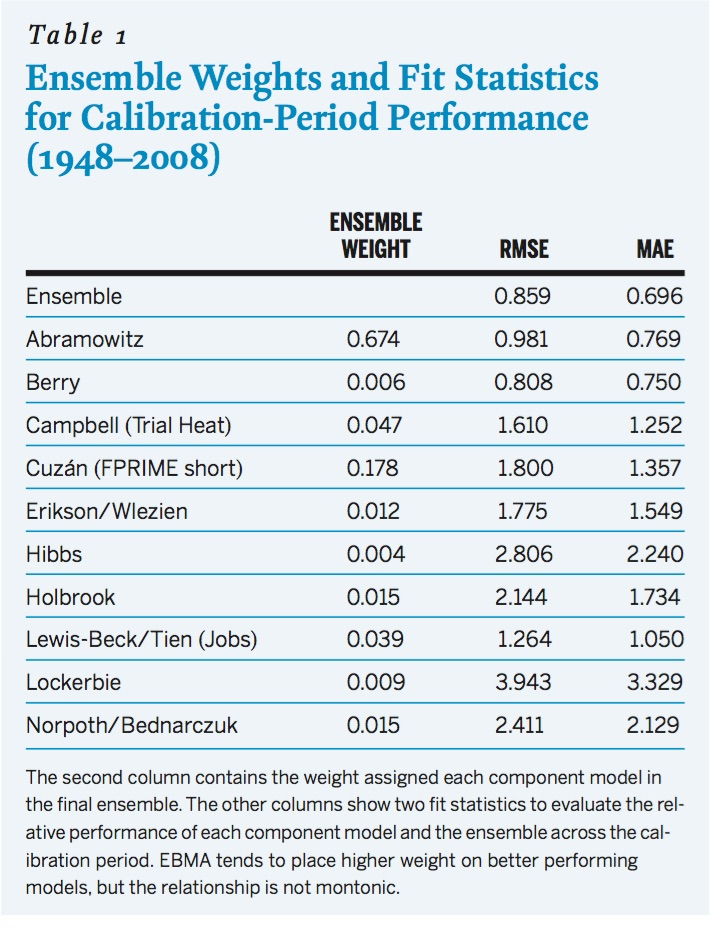
\includegraphics[scale=.2]{Figure2}
\end{center}

\bi
\item Forecast 50.2 [46.4, 52.5]
\item Outcome 51.3\%
\ei

\end{frame}

\begin{frame}
\frametitle{Truly Bayesian EBMA}

\bi
\item $t=[1, \ldots, T]$ is the number of predictions being made.
\item $k=[1, \ldots, K]$ is the number of models making predictions.
\item $y_t$ is the observed outcome for period $t$.
\item $\mathbf{X}=[\mathbf{x}_1, \mathbf{x}_2, \ldots, \mathbf{x}_K$], where  $\mathbf{x}_k = (x_{k1},x_{k2}, \ldots, x_{kT})$ is the vector of predictions made by model $k$.
\item $\boldsymbol{\tau} = [\tau_1, \tau_2, \tau_T]$ indexes which model actually generated observation $t$ such that $\tau_t \in [1, 2, \ldots, K] \forall t \in [1, 2, \ldots, T]$
\ei
\end{frame}

\begin{frame}
\begin{equation}p(y_{t}|\boldsymbol{\tau}, \boldsymbol{\sigma^2}, \mathbf{X}) \sim \sum_k^K N(x_{kt}, \sigma)\mathcal{I}(\tau_t=k),\end{equation} where $\mathcal{I}(\cdot)$ is the standard indicator function. The model is complete by specifying the following priors/hyperpriors.
\begin{gather}
\pi(\boldsymbol{\tau}) \sim \mbox{Multinomial}(\boldsymbol{\omega})\\
\pi(\boldsymbol{\omega}) \sim \mbox{Dirichlet}(\boldsymbol{\alpha})\\
\pi(\sigma^2) \sim (\sigma^2)^{-1} 
\end{gather}



\end{frame}



\begin{frame}



Let $\Theta$ be a $T$ by $K$ matrix holding a parameter indicating the latent probability such that $\theta_{tk}$ represents the that observation $t$ comes from model $k$. We calculate that, 

\begin{equation}
p(\theta_{tk} |\mathbf{X}, \mathbf{y}, \boldsymbol{\omega}) = \frac{\omega_kN(y_t|x_{tk}, \sigma)}{\sum_k^K\big(\omega_k N(y_t|x_{tk}, \sigma)\big)} 
\end{equation}

We then draw:

\begin{equation}
\tau_t |\Theta \sim \mbox{Multinomial}(\boldsymbol{\theta}_t)
\end{equation}

We then draw:

\begin{equation}
\boldsymbol{\omega}| \mathbf{\tau} \sim \mbox{Dirichlet}(\boldsymbol{\eta}),
\end{equation}
where $\eta_k=\alpha_k + \sum_{t=1}^T \mathcal{I}(\tau_t=k)$

\end{frame}

\begin{frame}

Finally, we need to calculate the conditional distribution for the posterior for the common variance term $\sigma^2$, which is

\begin{equation}\sigma^2 | \boldsymbol{\tau} \sim \mbox{Inv}.\chi^2\Big(\frac{T-1}{2}, \frac{\sum_{t=1}^T\big(y_t - \sum_{k=1}^K x_{tk}\mathcal{I}(\tau_t = k)\big) }{2}\Big)
\end{equation}

\end{frame}

\begin{frame}
\frametitle{Forecasting the 2016 election}

\begin{center}
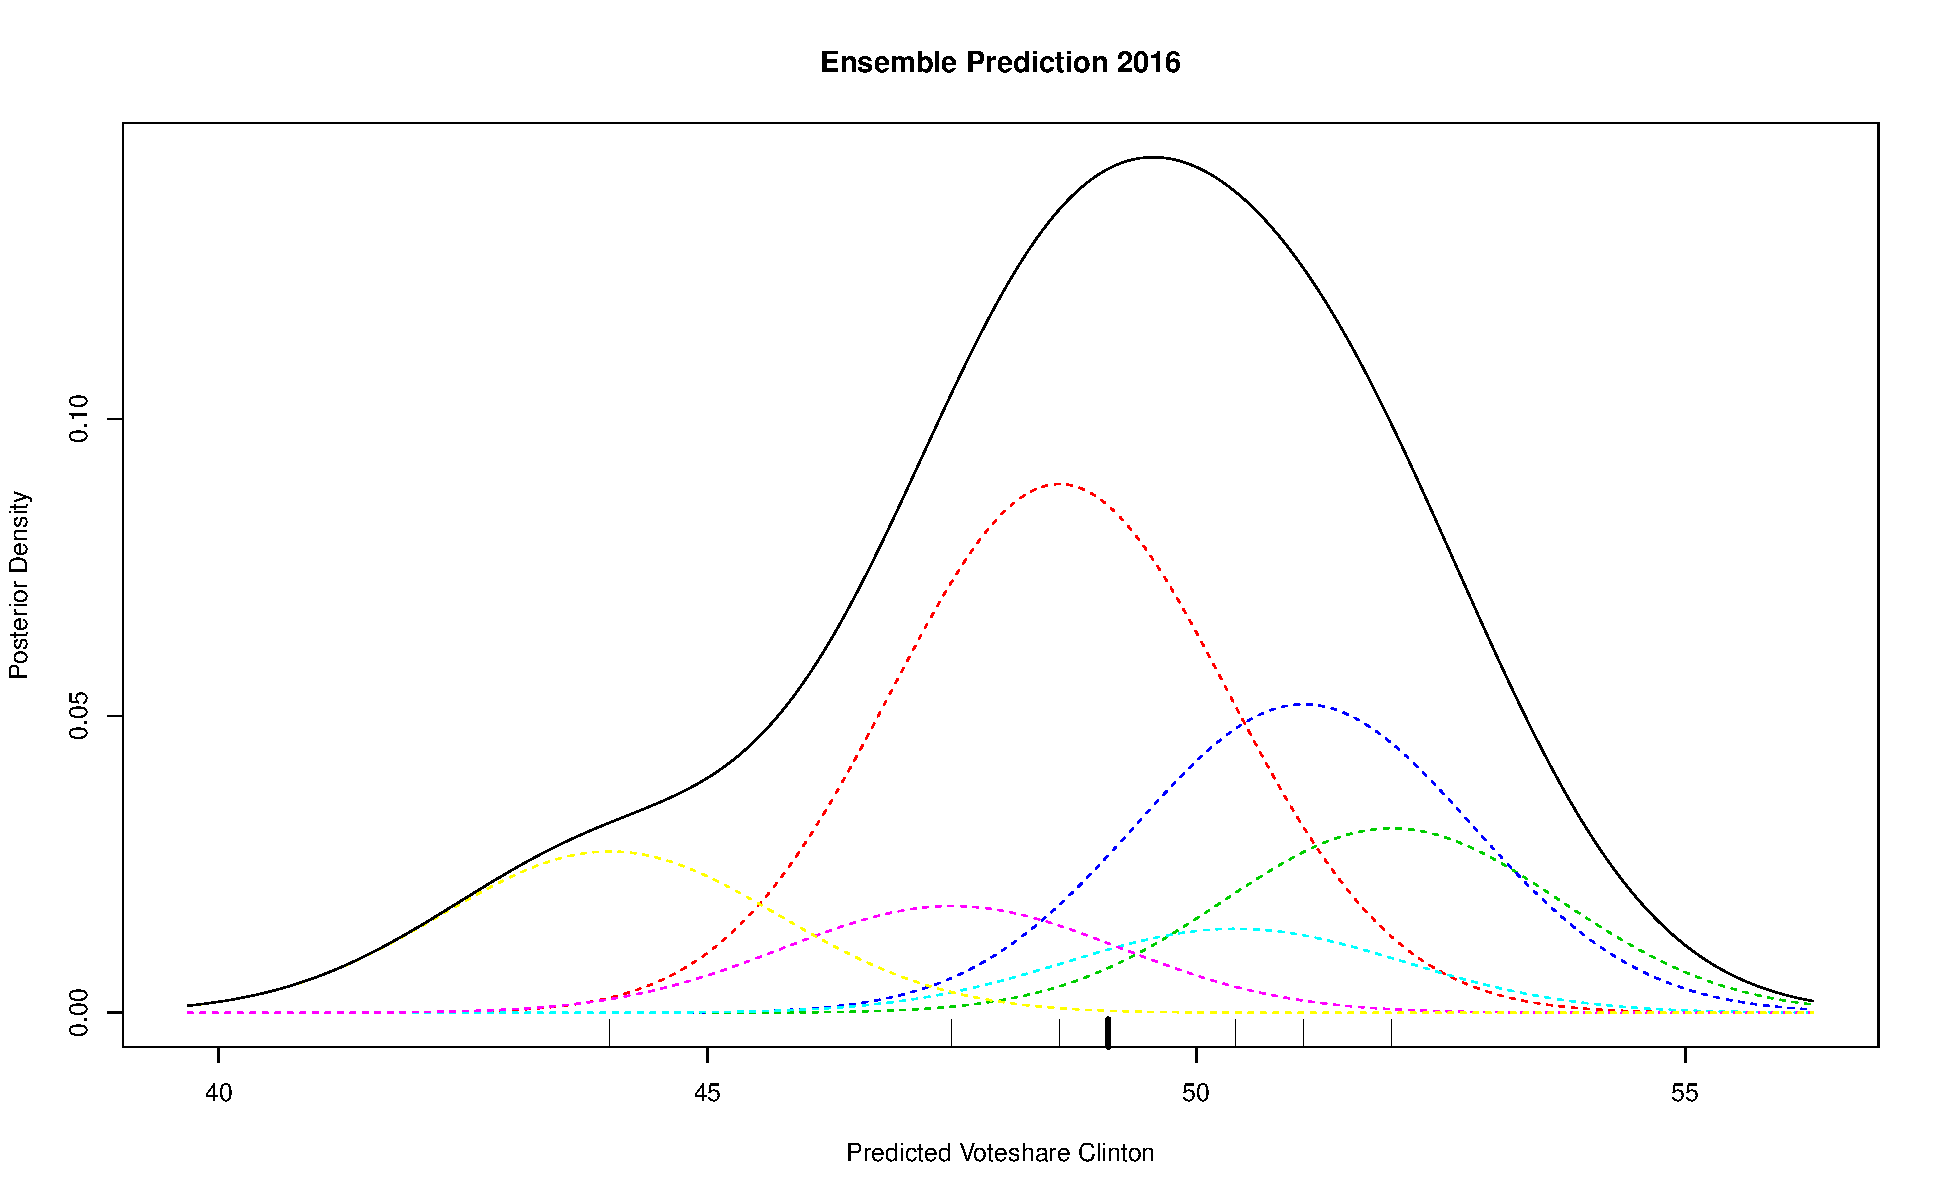
\includegraphics[scale=.38]{2016Forecast}
\end{center}

\end{frame}





\end{document}



\begin{frame}


\end{frame}





\end{document}

